% UNCONFIRMED REFRAME DRAFT v2, story structure (agent, 2026-11-01). Not
% reviewed by Dion or the group. The latest real draft is main.tex (box repo,
% 3b1a24c). Do not copy this file over it until the group agrees the reframe.
% What moved out of the main text: WHAT_MOVED.md and supplement_UNCONFIRMED.tex.
% v1 (same edits, old test-log structure): main_REFRAME_UNCONFIRMED_v1_logstyle.tex.
% Draft for SAFE @ AAAI 2027 (deadline 2026-11-03, 12:59 PM as listed on the
% submission site), AAAI-27 author kit
% (aaai2027.sty / aaai2027.bst, TemplateVersion 2027.1). Every number traces
% to a file under docs/ntire/ or to EXTENSIONS_TEST_REPORT.md.
\documentclass[letterpaper]{article} % DO NOT CHANGE THIS
\usepackage[submission]{aaai2027}  % DO NOT CHANGE THIS
\usepackage[hyphens]{url}  % DO NOT CHANGE THIS
\usepackage{graphicx} % DO NOT CHANGE THIS
\urlstyle{rm} % DO NOT CHANGE THIS
\def\UrlFont{\rm}  % DO NOT CHANGE THIS
\usepackage{natbib}  % DO NOT CHANGE THIS AND DO NOT ADD ANY OPTIONS TO IT
\usepackage{caption} % DO NOT CHANGE THIS AND DO NOT ADD ANY OPTIONS TO IT
\frenchspacing  % DO NOT CHANGE THIS
\usepackage{booktabs}
\usepackage{amsmath}
\usepackage{amssymb}

\pdfinfo{
/TemplateVersion (2027.1)
}

\setcounter{secnumdepth}{1} % the template allows 1 or 2

\newcommand{\fov}{\mathrm{FOV}}

% TITLE: open group choice. The text now uses one term, field of view of
% each view, which fits this title. Option 2 (Unequal Scales) would need the
% term changed to match.
\title{Equal Pixels, Unequal Views:\\Field of View Limits Robust AI-Generated Image Detection}
\author{Anonymous Submission}
\affiliations{}

\begin{document}
\maketitle

\begin{abstract}
AI-generated image detectors commonly score fixed-size crops taken at native
resolution, following the forensic advice to avoid resizing. A fixed-size crop
shows less of a larger image, so on large images the detector sees far less of
the scene than it did in training. We show that giving a frozen, crop-trained
DINOv2 detector the whole image instead improves robustness with no
retraining. On the hard validation split of the NTIRE 2026 Robust
AI-Generated Image Detection challenge, robust AUC rises from 0.886 to 0.963.
On large degraded images from the held-out AIGIBench SocialRF benchmark, it
rises by 8 to 9 points. Controlled experiments show that the gain comes from a
wider field of view in each input, the share of the image one input shows,
and not from tiling more of the image with extra crops at the same scale.
Downscaling the image before cropping widens each crop and helps DINOv2 on
both datasets, and CLIP and the public detector B-Free on SocialRF. Stronger
downscales may also weaken the degradation itself. The gain grows with
degradation strength and image size, while on large clean images whole-image
input lowers clean AUC. Every test was pre-registered. We also report two
label leaks in public benchmarks.
\end{abstract}

\section{Introduction}
\label{sec:intro}

Deployed detectors of AI-generated images see what social platforms deliver:
images that have been recompressed, resized and filtered, at every size. A
detector must turn each one into a fixed-size input. Forensic work argues
that this step should not resize: ``Most of all, it is important
to avoid resizing'' because interpolation ``may erase the subtle
high-frequency traces left by the generation process''
\cite{corvi2023detection}. The usual answer is a fixed-size crop at native
resolution, which we call a \emph{window}, scored once or several times with
the scores averaged
\cite{corvi2023detection,li2025safe,guillaro2025bfree,konstantinidou2025texturecrop}.

A fixed-size window keeps pixel count equal across images. It does not keep
field of view equal. We call each square input the model scores a \emph{view}, and define
its field of view as the share of the image's short side it shows: a window of
side $s$ on an image with short side $h$ has $\fov = s/h$. A 200-pixel window covers 39\% of the short
side of a 512-pixel image and 5\% of a 4000-pixel one, so the larger the
image, the less of it each view shows. FixRes \cite{touvron2019fixres}
describes a related effect in image classification, where a change in
apparent object size between training and test costs accuracy (``networks do
not have built-in scale invariance''). That account, a covariate
shift \cite{shimodaira2000covariate} in the input, predicts that a detector
does best when the test view matches the training view.

Our detector fits this account. We built it for the NTIRE 2026 Robust AI-Generated Image Detection challenge
\cite{gushchin2026ntire}. All 407k training images have a short side of at
most 512 pixels, so a 200-pixel window at native scale showed at least 39\%
of the short side. Augmentation could crop a window further,
to no less than 20\%, and always enlarged what remained. On the organisers'
hard validation split a native window shows as little as 5\%, and robust AUC
fell as native image size grew. Three pre-registered method changes aimed at
the degradations did not help. Showing the whole image did, by 7 to 9 points
per branch, with no retraining. The limit is the field of view of each view.
Pixel count matters little, and so does \emph{coverage}, the share of the
image that all views show together when we tile it with more windows of the
same size.

\paragraph{Contributions.}
\begin{itemize}
\item A diagnosis. For our vision transformer detectors on degraded images,
  the field of view of each view limits robust AUC, and pixel count does not.
  Whole-image input recovers 7 to 9 points per branch with no retraining, and
  the gain is not a resolution shortcut (Secs.~\ref{sec:diagnosis}
  and~\ref{sec:controls}).
\item A mechanism. Controlled experiments separate field of view, coverage
  and degradation removal. The gain comes from a wider field of view in each
  view, not from tiling more of the image with same-size windows. A 2x
  downscale removes no
  measurable degradation for DINOv2 and a little for CLIP, and stronger
  downscales may also reduce it. The gain grows with degradation level and
  image size (Sec.~\ref{sec:decomp}).
\item Reach and baselines. The downscale gain holds for DINOv2, CLIP and
  B-Free, a public detector built on native-resolution traces. Whole-image
  input beats three alternatives: a native window with no enlargement,
  multi-scale training, and a learned combiner over nine windows (Secs.~\ref{sec:training}
  and~\ref{sec:heldout}).
\item Where it stops. On large clean images whole-image input costs clean
  AUC, for B-Free as for our detectors, and we cannot yet say why. Every
  detector we tested is a vision transformer. Along the way we found two label
  leaks in public benchmarks: a file-format and size confound in AIGIBench
  CommunityAI \cite{li2025aigibench}, and a non-monotone size leak in the
  resized RAISE reals commonly paired with Synthbuster
  \cite{bammey2024synthbuster} (Sec.~\ref{sec:leaks}).
\end{itemize}

Whole-image input is not new. The NTIRE 2026 winner resizes the whole image at
inference ``to preserve the global spatial context'', the fifth-placed team
calls its preprocessing ``squish'' \cite{gushchin2026ntire}, and
AI-GenBench \cite{pellegrini2025aigenbench} finds resize ``often preferable''
to multi-crop for CLIP and DINOv2 backbones. Each gives a one-line rationale:
AI-GenBench notes that multi-crop uses ``only partial content information'',
and the NTIRE entries cite global context or full image content. None
separates each view's field of view from coverage, pixel count
and degradation removal, or tests the rationale. Our contribution is that
test and the evidence around it. We also show where the advice to avoid
resizing still holds.

\section{Related work}
\label{sec:related}

\paragraph{Crop, don't resize.} \citet{corvi2023detection} recommend
training on native patches cropped without resizing and deciding on the whole
image by fusion. SAFE \cite{li2025safe} replaces
down-sampling with a crop and reports that the resize ``indeed diminishes the
subtle artifact features''. B-Free \cite{guillaro2025bfree} trains on
504-pixel crops and averages native-resolution crops at test time.
SPAI \cite{karageorgiou2025spai} learns a spectral model so that any
resolution can be scored without resizing. TextureCrop \cite{konstantinidou2025texturecrop}
selects textured native crops and notes that preprocessing loss grows with
native resolution. HiDA-Net \cite{mu2026hidanet} tiles the full image and
reports 84.2\% accuracy from its global view alone against 96.1\% with tiles.
All of these reason about high-frequency traces. SAFE's own ablation is
useful context for us: its CNN scores a centre crop and the full native image
about equally, so a low-level detector does not appear to depend on field of
view.

\paragraph{Resize can win.} AI-GenBench \cite{pellegrini2025aigenbench}
reports resize at least as good as five-crop for fine-tuned DINOv2 ViT-L/14
(94.24 against 93.44 AUROC) and clearly better for CLIP (92.04 against 87.66).
In AIGIBench's test-time comparison \cite{li2025aigibench}, the one CLIP-based
detector does better with resize while all five low-level detectors do better
with crops. \citet{cozzolino2024raising} resize the short side
before a centre crop.\footnote{In their released code,
\url{https://github.com/grip-unina/ClipBased-SyntheticImageDetection}.} WaRPAD \cite{choi2025warpad} rescales the whole image to
a fixed square before tiling it, which holds each tile's field of view
constant, although the paper motivates it differently. GlobalForge \cite{cui2026globalforge}
reports the opposite of our test-time result on clean data: a UnivFD probe
trained with centre crops loses about 9 balanced-accuracy points (67.9 to
58.7, their Fig.~2) when tested with resize. We return to this in Sec.~\ref{sec:heldout}.

\paragraph{Scale and size as confounds.} \citet{grommelt2024fakeorjpeg}
show that JPEG quality and image size
separate real from fake in GenImage, and note in one sentence that
``detectors employing cropping to achieve a uniform input size are still
subject to bias in terms of object size''. Their concern is a size shortcut
correlated with the label. Ours is the reverse case: size is uninformative in
training and the detector still fails across sizes at test time. \citet{rajan2025aligned}
show that random resized crops inject
resampling signals when real and fake sizes differ, and BIAS-ID \cite{ricker2026biasid}
measures detector score shifts under such transformations. FixRes \cite{touvron2019fixres}
is the closest precedent. Sec.~\ref{sec:decomp} shows that its train-test
account fits our data at the level of a single view.

\section{Setup}
\label{sec:setup}

\paragraph{Data.} We train on 407,223 images: the NTIRE 2026 training shards,
COCO and Open Images reals, and paired real and generated images from several
open and commercial generators. Every training image has a short side of 200 to
512 pixels (median 512, and 384 or more for 95\% of images). We evaluate on the organisers' labelled splits:
\texttt{ntire\_val} (10,000 images, half distorted), \texttt{ntire\_val\_hard}
(2,500, half distorted) and the public test split \texttt{ntire\_test}
(2,500). Robust AUC is the ROC AUC over distorted images, and clean AUC is
over undistorted ones, following the challenge \cite{gushchin2026ntire}.

\paragraph{Models.} Two branches built on DINOv2-L/14 with
registers \cite{oquab2024dinov2,darcet2024registers}, all 24 blocks
fine-tuned, mean-pooled patch tokens, 0.91B parameters in total. Branch A is
one tower at a 512-pixel input, trained for 2 epochs. Branch B concatenates
two towers at 224 pixels, trained for 3 epochs. Each source image yields one
clean view and ten degraded views drawn from a pool of 26 operations in six
families, chained up to five deep, including a neural codec \cite{balle2018hyperprior}
and a downscale applied before the window is taken. The loss is
class-balanced cross-entropy plus a degradation-prediction term (weight 0.3)
and clean-degraded consistency terms on the outputs (KL) and hidden
features (MSE), each at unit weight. The schedule is cosine with 3\% warm-up, with weight
averaging \cite{izmailov2018swa} over the last quarter. On one RTX 4090 the
squish-trained branches took about 19 hours (B) and 29 hours (A).

\paragraph{Views, field of view and coverage.} A \emph{view} is one
square input to the model: a region of the image resized to the branch's input
size. A detector may score several views of one image and average their
logits. The \emph{field of view} of a view is the share of the image's short
side it shows. \emph{Coverage} is the share of the image area that all views
of one image show together. A 200-pixel window cut after the image is
downscaled by a factor $k$ has $\fov = 200k/h$. Downscaling therefore widens
every view and leaves coverage unchanged, while tiling more of the image with
same-size windows raises coverage and leaves each view unchanged.

The \emph{crop} policy takes one 200-pixel window at native resolution (the
centre window at test time) and resizes it to the branch's input size. Images
with a short side under 200 pixels are taken whole. The \emph{squish} policy
resizes the whole image to the input size, discarding aspect ratio: area
interpolation on the short side down to the input size when the image is
larger, then area interpolation to the square. Both policies give every image
the same number of input pixels. Under squish, field of view and coverage are
both 1. To vary the two one at a time, \emph{tiles}$(k, f)$ takes the centred
region holding a fraction $f$ of the image area, downscales it by $k$ with
area interpolation, covers it with 200-pixel windows, resizes each window to
the input size and averages the logits. $f$ sets coverage and $k$ sets each
view's field of view.

\paragraph{Fusion and selection.} The two branches' logits are z-scored and
combined as $w z_A + (1-w) z_B$. The z-score parameters and the weight $w$ are
fitted on \texttt{ntire\_val} alone, by the mean of robust and clean AUC. For
the squish models the choice between final and averaged weights is made the
same way. For the crop models we kept the choice made earlier on both
validation splits. The fitted weights were $w = 0.50$ for crop and $w = 0.55$
for squish.

\paragraph{Statistics.} All intervals are 95\% percentile intervals from 2,000
paired bootstrap resamples, stratified by label and distortion status, with
the same resample indices for every model being compared.

\paragraph{Protocol.} The test split was read once with the crop fusion
(2026-10-04). We then committed a pre-registration of the squish study,
which allowed exactly one more read of the test split, before training any
squish model. Every later test in this paper was registered before any of
its numbers existed, and none read the test split again. The supplement
lists every registered test, its outcome and where it is reported, including
those that failed or could not be identified. We mark the few numbers that
were not registered as exploratory. We chose the squish policy
after seeing its effect on \texttt{ntire\_val\_hard}, so its numbers on that
split are optimistic, and we label them \emph{selection split}. The external benchmarks and the test read
carry the held-out evidence. Code, the pre-registration and per-image scores
will be released with the paper.

\section{Equal pixels, unequal views}
\label{sec:diagnosis}

\begin{table}[t]
\centering
\small
\begin{tabular}{lrrrr}
\toprule
split & n & p5 & p50 & p95 \\
\midrule
train, native & 407,223 & 0.391 & 0.391 & 0.521 \\
train, window taken & 220,000 & 0.391 & 0.468 & 1.000 \\
train, after second crop & 220,000 & 0.296 & 0.415 & 0.942 \\
\texttt{ntire\_val} & 10,000 & 0.100 & 0.312 & 0.893 \\
\texttt{ntire\_val\_hard} & 2,500 & 0.112 & 0.298 & 0.784 \\
\bottomrule
\end{tabular}
\caption{Field of view of the 200-pixel window ($200/$short side).
\emph{Window taken} is the window as the trainer cuts it, on 20,000 seeded
training images with 11 views each. A downscale before the window widens the
field of view: 24.9\% of views exceed 0.521 and 6.3\% show the whole short
side. A crop after the window narrows 18\% of views below 0.391, to no less
than 0.195, and enlarges them back. On \texttt{ntire\_val\_hard}, 70.8\% of
images fall below 0.391, and the smallest views (0.05) are about 4 times
narrower than any training view.}
\label{tab:fov}
\end{table}

Table~\ref{tab:fov} shows how much of each image the window covers. In
training a native-scale window shows 39 to 52\% of the short side.
Augmentation widens some views and narrows others, but never below 20\%. On \texttt{ntire\_val\_hard} the median
is 30\%, and one image in twenty gets 11\% or less. Under the crop policy,
fused robust AUC on \texttt{ntire\_val\_hard} falls from 0.911 for images
with a short side of 80 to 336 pixels to 0.865 for images above 752 pixels.
Figure~\ref{fig:size} shows the same fall in eight equal-count bins.

\begin{figure}[t]
\centering
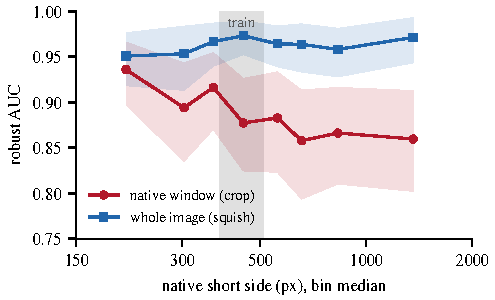
\includegraphics[width=\columnwidth]{fig_size}
\caption{Fused robust AUC on the distorted rows of \texttt{ntire\_val\_hard}
(selection split) in eight equal-count bins of native short side, with 95\%
bootstrap bands. Red: the crop-trained fusion under its 200-pixel window.
Blue: the fusion trained under squish. Grey: the native short sides of the
training images.}
\label{fig:size}
\end{figure}

To separate field of view from pixel count, we scored the two frozen
crop-trained branches under four test-time presentations
(Table~\ref{tab:probe}). \emph{grid9} averages nine 200-pixel native windows,
nine times the pixels at the same field of view. \emph{fov3} first downscales
the short side to 600 pixels and then takes the nine windows, which raises the
field of view to $1/3$. \emph{squish} shows the whole image once.

\begin{table}[t]
\centering
\small
\setlength{\tabcolsep}{4pt}
\begin{tabular}{llrrr}
\toprule
branch & presentation & views & robust & clean \\
\midrule
A (512) & centre window & 1 & 0.8561 & 0.9912 \\
        & grid9 & 8.9 & 0.8495 & 0.9978 \\
        & fov3 & 8.9 & 0.8703 & 0.9977 \\
        & squish & 1 & \textbf{0.9482} & 0.9906 \\
\midrule
B (224) & centre window & 1 & 0.8872 & 0.9801 \\
        & grid9 & 8.9 & 0.9049 & 0.9931 \\
        & fov3 & 8.9 & 0.9215 & 0.9942 \\
        & squish & 1 & \textbf{0.9599} & 0.9886 \\
\bottomrule
\end{tabular}
\caption{Frozen crop-trained branches on \texttt{ntire\_val\_hard} (fit
split) under test-time presentations. More pixels at the same field of view
(grid9) help B by 1.8 points and cost A 0.7. Raising the field of view helps
in proportion.}
\label{tab:probe}
\end{table}

More pixels at the same field of view do little: grid9 gains 1.8 robust
points on B and loses 0.7 on A. Gains rise with field of view: fov3 gains 1.4
and 3.4 points, and squish gains 9.2 and 7.3. Squish uses one view and the
same pixel count as the centre window. On B the paired interval for the
squish gain is [+0.057, +0.090]. With z-scores and weight fitted on
\texttt{ntire\_val}, the fused robust AUC rises from 0.886 to 0.963 and the
true positive rate at 1\% false positive rate from 0.516 to 0.752. Clean AUC
moves by $-0.001$ on A and $+0.009$ on B.

Squish changes three things at once. It raises coverage to the whole
image, widens the field of view of its one view, and averages any degradation
over more pixels. Sec.~\ref{sec:decomp} separates the three, after we rule out
the simplest explanation.

\section{It is not a resolution shortcut}
\label{sec:controls}

Squish does not hide native resolution. A small image arrives upsampled and
soft, a large one downsampled and sharp, so a model could read size from the
pixels. Four checks argue against this. Native short side scores an AUC of
only 0.528 against the label on the training set, so the training data does
not reward reading size. Within equal-count deciles of native short side,
where the resize factor is nearly constant, squish beats the centre window in
10 of 10 deciles on branch B (size-weighted robust AUC 0.888 to 0.964, against
7.3 points pooled). When we band-limit the squished input to 160 pixels, so
native resolution can no longer be read from it, branch B keeps +7.2 of its
+7.3 points. Branch A keeps +5.7 of +9.2, the expected cost of removing real
detail from a 512-pixel input. Last, the challenge's validation splits add
crops, downscaling and perspective transforms that change native size
\cite{gushchin2026ntire}. On rows that received only photometric transforms
(median short side 784 pixels) the gain is +9.0 points on A and +8.3 on B,
with intervals clear of zero.

Squish also stretches non-square images, which can introduce frequency
artefacts along one axis \cite{grommelt2024fakeorjpeg}. Two
aspect-preserving presentations, the centre square after resizing the short
side and a padded letterbox, keep 93 to 100\% of squish's gain on both
branches. Showing the whole short side drives the gain, not the stretch.

\section{What the gain is made of}
\label{sec:decomp}

This section uses the frozen crop-trained branches throughout.

\paragraph{Degradation and size.} We took the 6,250 undistorted images of the
two validation splits and applied JPEG (quality 90, 70, 30), Gaussian blur
($\sigma$ 0.5, 1, 2) or Gaussian noise ($\sigma$ 0.02, 0.05, 0.10) at native
resolution. The robust gain of squish over the centre window, averaged over
the three operations, rises from $-0.001$ with no degradation to $+0.029$ at
the heaviest level on branch A, and from $+0.004$ to $+0.027$ on B. Every
rise from none to heavy has an interval above zero, pooled and in every size
bucket. The rise is largest above 752 pixels ($+0.049$ on both branches). On
undistorted images up to 736 pixels the two policies differ by at most
0.002. The levels are not matched in strength across operations, so we do
not rank the operations.

\paragraph{Coverage against downscale.} The images used here have a short
side of at least 800 pixels. We scored \emph{tiles}$(k, f)$ at
$k \in \{1, 2\}$ and $f \in \{0.25, 0.5, 1\}$, so every window is a
200-pixel window like those in training. The coverage effect $d_F$ is the
gain from $f = 0.25$ to $f = 1$ averaged over $k$. The downscale effect $d_K$
is the gain from $k = 1$ to $k = 2$ averaged over $f$. On NTIRE (4,068 images,
1,235 distorted, selection split) both effects are above zero on both branches
(Table~\ref{tab:decomp}). On large degraded SocialRF images, which no model
was trained or selected on, coverage does nothing: at a fixed downscale,
showing the whole image instead of its central quarter changes robust AUC by
less than 0.01. The downscale helps by 2.3 to 5.5 points at every coverage
level, more than on NTIRE. Covering the whole image after a 4x downscale,
\emph{tiles}$(4, 1)$, is within 0.003 of squish on NTIRE and at least as good
on SocialRF (A 0.973 against 0.958, B 0.966 against 0.962). Figure~\ref{fig:tiles} shows all cells: the lines are nearly flat in
coverage, and downscaling lifts them.

\paragraph{Field of view, not degradation removal.} A downscale by 2 does
two things. It averages neighbouring pixels, which can remove degradation,
and it doubles each window's field of view. To split them we downscaled each
region by 2 and enlarged it back before cutting the windows. These windows
have the field of view of \emph{tiles}$(1, f)$ and the averaged pixels of
\emph{tiles}$(2, f)$. The difference from \emph{tiles}$(1, f)$ is the
degradation-removal part $d_A$, and the rest of $d_K$ is the field-of-view
part $d_V$. On both datasets and both branches $d_A$ is at most 0.004 in size,
with an interval that includes zero, and $d_V$ carries the whole effect. The
round-trip windows are about four times as many per image as those of
\emph{tiles}$(2, f)$, so part of $d_V$ may come from mean pooling diluting
fewer strong windows. This test cannot separate the two.

\paragraph{Stronger downscales.} Squish downscales large images 5 to 18
times, far more than 2. To look at stronger factors we took 2,833 undistorted
NTIRE images with a short side of at least 800 pixels and applied heavy JPEG
(quality 30), blur ($\sigma = 2$) or noise ($\sigma = 0.10$) either before or
after downscaling by $k$, then scored \emph{tiles}$(k, 1)$. $R(k)$ is robust
AUC with the degradation applied before the downscale minus after it, so a
positive $R$ means the downscale weakened the degradation. On branch A,
$R(2) = +0.022$ [+0.019, +0.026] and $R(4) = +0.036$. On B they are +0.007
[+0.005, +0.008] and +0.013. $R(4)$ exceeds $R(2)$ on both branches, and noise,
the degradation a downscale should average away most easily, gives the largest
$R$ on both (A: +0.030 at 2x, +0.047 at 4x). This fits a downscale that also
reduces the degradation, more so at stronger factors. It is not proof. The
same degradation may hurt more when applied to a smaller image, JPEG blocks
shrink with the image, and at 2x the round trip above found no removal. We
claim only that stronger downscales may also reduce the degradation.

\paragraph{A mismatch in each view.} No training view showed less than
20\% of the short side, and none at native scale less than 39\%
(Table~\ref{tab:fov}), while a 200-pixel window on a 3,000-pixel photo shows
7\%. Downscaling moves each view's field of view back toward the trained
range, and squish sets it to 1, inside that range. This is a train-test
mismatch in each view's field of view, as FixRes describes, not in the image
as a whole. It is not the whole story. In the bin of Figure~\ref{fig:size}
whose short sides (416 to 496 pixels) lie inside the training range, the crop
fusion still scores 0.877 against 0.973 for squish. Many of these images were
downscaled from larger originals, so objects in them may appear at a
different size than in training.

\paragraph{CLIP.} We repeated the decomposition on three short CLIP
ViT-L/14 runs trained on crops (Sec.~\ref{sec:training}), on the same SocialRF
images. Downscaling helps by 5.4 to 7.6 points and coverage does nothing, as
on DINOv2. Most of the gain is the field-of-view part ($d_V$ +0.041 to
+0.063), but on CLIP the round trip also removes a little degradation ($d_A$
+0.011 to +0.014, above zero on every seed). No measurable removal at 2x is
therefore a DINOv2 result.

\begin{table}[t]
\centering
\footnotesize
\setlength{\tabcolsep}{2pt}
\begin{tabular}{llrrrrr}
\toprule
data & branch & $d_F$ & $d_K$ & $d_A$ & $d_V$ & $R(4)$ \\
\midrule
NTIRE & A & +0.005* & +0.014* & $-0.002$ & +0.016* & +0.036* \\
      & B & +0.011* & +0.008* & $-0.001$ & +0.010* & +0.013* \\
SocialRF & A & $-0.004$ & +0.050* & +0.001 & +0.049* & n/a \\
         & B & +0.001 & +0.027* & +0.004 & +0.023* & n/a \\
\bottomrule
\end{tabular}
\caption{Decomposition of the robust gain, frozen crop-trained branches,
images with a short side of at least 800 pixels. $d_F$: coverage, from 25\% to 100\% of the image. $d_K$: downscale by 2.
$d_A$ and $d_V$ split $d_K$ into degradation removal and field of view
($d_A + d_V = d_K$). $R(4)$: robust AUC with heavy degradation applied before
a 4x downscale minus after it, on 2,833 undistorted NTIRE images. NTIRE rows are from the selection split. SocialRF rows
use our degradation chains. * marks a 95\% interval that excludes zero.}
\label{tab:decomp}
\end{table}

\begin{figure*}[t]
\centering
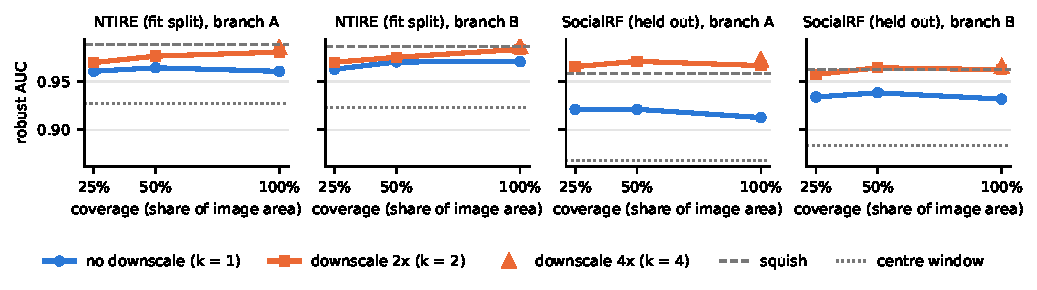
\includegraphics[width=\textwidth]{fig_tiles}
\caption{Robust AUC of \emph{tiles}$(k, f)$ for the frozen crop-trained
branches on images with a short side of at least 800 pixels. Moving right
tiles more of the image with same-size windows (coverage). Moving up a line downscales
the image first, widening each view. On held-out SocialRF the lines are flat
in coverage and the downscale carries the gain. Dashed: squish. Dotted: the
centre window.}
\label{fig:tiles}
\end{figure*}

\section{Training and baselines}
\label{sec:training}

\paragraph{Training under whole-image input.} In short training runs (one tower,
one epoch on a quarter of the training set, three seeds), squish-trained
models beat crop-trained ones by +0.083 [+0.062, +0.105], +0.093 [+0.072,
+0.115] and +0.078 [+0.057, +0.102] robust AUC on \texttt{ntire\_val\_hard},
with clean AUC within noise. We then trained the full branches under squish
(Table~\ref{tab:branches}). They match the test-time change on robust AUC (A:
0.943 against 0.948, B: 0.959 against 0.960) and add a little clean AUC. The
fused squish-trained models reach 0.960 robust and 0.995 clean, against 0.886
and 0.990 for the crop fusion: +0.074 [+0.058, +0.091]. The size gradient is
gone: across the eight bins of Figure~\ref{fig:size} the squish fusion stays
between 0.951 and 0.973. In the short runs, training under squish adds 4 to 6
points beyond the test-time change, with DINOv2 and with CLIP (an
exploratory comparison). The full branches show no such gap. They
differ from the short runs in training length, number of views per image and
loss terms, and we cannot say which of these closes the gap.

\begin{table}[t]
\centering
\small
\setlength{\tabcolsep}{4pt}
\begin{tabular}{llcc}
\toprule
branch & model & robust & clean \\
\midrule
A & crop-trained & 0.8561 & 0.9913 \\
  & crop-trained, squish at test & 0.9482 & 0.9906 \\
  & squish-trained & 0.9425 & 0.9934 \\
\midrule
B & crop-trained & 0.8873 & 0.9801 \\
  & crop-trained, squish at test & 0.9599 & 0.9886 \\
  & squish-trained & 0.9589 & 0.9898 \\
\bottomrule
\end{tabular}
\caption{Per branch on \texttt{ntire\_val\_hard} (selection split). Training under
squish adds nothing to robust AUC beyond presenting the whole image to the
crop-trained model. Paired gains over crop-trained: A +0.092 and +0.086, B
+0.073 and +0.072, all intervals clear of zero. The crop-trained rows were
rescored for this table and differ from Table~\ref{tab:probe} by at most
0.0001.}
\label{tab:branches}
\end{table}

\paragraph{A second backbone.} We repeated the short-run comparison with a CLIP
ViT-L/14 tower \cite{radford2021clip} in place of DINOv2, every other setting
unchanged. Over three seeds, training under squish beat crop by +0.139 to
+0.150 robust AUC, with clean AUC unchanged, and showing the crop-trained
checkpoints the whole image gained +0.094 to +0.111 at test time alone, every
interval clear of zero. Both gains grow with size: at test time, +0.168 above
752 pixels against +0.057 below 336. CLIP's crop-trained short runs are weaker
than DINOv2's (0.748 robust against 0.799) and gain more.

\paragraph{Is the crop baseline fair?} The crop policy enlarges its
200-pixel window to the input size, 1.12 times for B and 2.59 times for A,
and averaging native windows may dilute one informative window. We checked
both. A 224-pixel native window fed at 224, with no enlargement, scores
within 0.013 of the 200-pixel window, and the squish-trained short runs beat it
by +0.077 on average over three seeds. At 512 pixels a native 512-pixel
window beats the enlarged 200-pixel one by +0.042 [+0.025, +0.058] at one
seed, but it also has 2.56 times the field of view. A 196-pixel window
fed at 196 pixels has the field of view of the enlarged 200-pixel window
without the enlargement, and separates the two. On 630 large degraded images
the native 512-pixel window leads by 0.059. The field-of-view part is +0.048
[+0.022, +0.072]. The enlargement part is +0.011 [$-0.014$, +0.037], too
uncertain to call, so whether enlargement handicaps branch A's crop baseline
remains open.
Multi-scale training with random resized crops (area 0.20 to 1.00) closes 73
to 81\% of the gap between crop and squish, and squish stays ahead by +0.019
on average, every interval clear of zero. On the full frozen branches, a
learned attention combiner over the nine native windows, fitted on
\texttt{ntire\_val}, gains about 3 points over averaging them. Squish, which
is not fitted, still beats it by +0.069 [+0.052, +0.087] on A and +0.023
[+0.011, +0.036] on B, and ties it on B for images below 336 pixels.

\section{Held-out evidence and where it stops}
\label{sec:heldout}

\paragraph{External benchmarks.} We scored three external benchmarks that no
model was trained or selected on, after removing any image whose content
digest matched an NTIRE image: AIGIBench SocialRF and CommunityAI
\cite{li2025aigibench}, and Synthbuster with RAISE-1k reals
\cite{bammey2024synthbuster,dangnguyen2015raise}. All three are clean, so we
report pooled AUC on the files as distributed, on every file re-encoded as
JPEG at quality 95, and on every file passed through one seeded chain from
our degradation pool. That last reading is our own synthesis, not the
organisers'.

\begin{table*}[t]
\centering
\small
\begin{tabular}{lccc}
\toprule
 & SocialRF & CommunityAI & Synthbuster \\
\midrule
n (real/fake) & 2994/3000 & 6000/6000 & 994/8996 \\
short side p50 & 1366 & 500 & 833 \\
size-label AUC & 0.694 & 0.916 & 0.519 \\
format-label AUC & 0.500 & 1.000 & 0.555 \\
\midrule
crop fusion & 0.9633 & 0.9809 & 0.9995 \\
squish fusion & 0.9776 & 0.9920 & 0.9984 \\
difference & +0.014 & +0.011 & $-0.001$ \\
\quad 95\% CI & [+0.010, +0.018] & [+0.009, +0.013] & [$-0.002$, $-0.001$] \\
\midrule
size-matched, JPEG 95 & +0.016 & +0.005 & n/a \\
\quad 95\% CI & [+0.009, +0.024] & [$-0.002$, +0.012] & \\
degraded (ours) & +0.085 & +0.070 & +0.024 \\
\bottomrule
\end{tabular}
\caption{External benchmarks, fused AUC. Size-matched is the size-weighted AUC
within deciles of native short side. It cannot be computed on Synthbuster
because no decile holds both classes (Sec.~\ref{sec:leaks}).}
\label{tab:external}
\end{table*}

Table~\ref{tab:external} gives the results. On SocialRF, squish wins on the
files as distributed, after JPEG re-encoding, and within size deciles, and on
its large degraded images the gain comes from the downscale
(Sec.~\ref{sec:decomp}). On CommunityAI the pooled gain is confounded: every
real image is a JPEG and every fake a PNG, and native size alone separates
the classes with AUC 0.916. The size-matched gain on the re-encoded files does
not clear zero ([$-0.002$, +0.012]). On Synthbuster squish loses by 0.001,
with both fusions near ceiling. Under our degradation chains squish wins on
all three sets, by 2.4 to 8.5 points.

\paragraph{The second test read.} Table~\ref{tab:test} gives both reads of
the public test split. Read 1 used the crop fusion as frozen on 2026-09-23.
Read 2 used the squish fusion as frozen before any squish model was scored on
test, and our pre-registration allows no third read. Robust AUC rose by
+0.062 [+0.040, +0.083] and clean AUC fell by 0.014 [0.006, 0.024]. On robust
AUC the squish fusion would sit between the sixth- and seventh-placed
challenge entries on the open test, where the crop fusion was below all nine.
We were not a challenge entry and make no ranking claim. The leading entries
use far more compute, such as committees of DINOv3 models at 512 pixels on 32
A100 GPUs \cite{gushchin2026ntire}.

\begin{table}[t]
\centering
\small
\begin{tabular}{lcccc}
\toprule
read & robust & clean & AUC & TPR@1\% \\
\midrule
1, crop & 0.7931 & 0.9856 & 0.9108 & 0.289 \\
2, squish & 0.8547 & 0.9715 & 0.9211 & 0.300 \\
\bottomrule
\end{tabular}
\caption{The two reads of \texttt{ntire\_test} (2,500 images). Read 1's fusion
weight was fitted on both validation splits ($w = 0.45$), read 2's on
\texttt{ntire\_val} alone.}
\label{tab:test}
\end{table}

\paragraph{The clean cost.} The clean loss on the test split has one source.
Clean AUC of branch A on test images with a short side above 1100 pixels
falls from 0.974 under crop to 0.880 under squish (366 images). Below 1100
pixels, and on branch B at every size, the change is under 1.3 points. The
fake images drive it: their mean score under squish falls with size. The
validation splits do not show this cost, and the test split carries no
generator labels. Synthbuster, which has them, shows no single location
either. The two A models also differ in weight averaging and training round,
not only in input policy. We tried to remove the cost with a per-image mix of
squish and grid9, weighted by the branch's predicted degradation. It lost
robust AUC against squish alone ($-0.005$ [$-0.010$, $-0.001$]), so we did
not spend a test read on it. Our hypothesis is the trade-off the forensic
literature predicts: a clean, large generated image keeps fine traces at
native resolution, and reducing it to 512 pixels discards them. This would
also reconcile our result with GlobalForge \cite{cui2026globalforge} and
TextureCrop's CLIP results \cite{konstantinidou2025texturecrop}, both
measured on clean data. Once blur, compression or downscaling has damaged the
traces, the detector has to judge content, and each view needs a wider field of
view. We have not tested this hypothesis directly.

\paragraph{Public detectors.} UnivFD \cite{ojha2023univfd}, a linear probe on
CLIP ViT-L/14 features trained on 224-pixel crops, is at chance on NTIRE data
under every presentation (robust AUC 0.49 to 0.51 on the hard split), so it
says nothing either way. B-Free \cite{guillaro2025bfree} is a DINOv2-B with
registers that averages five 504-pixel windows taken at native
resolution.\footnote{Model size and window count from the released weights
and code, \url{https://github.com/grip-unina/B-Free}.} We scored it with its
authors' pipeline (native), at its own training field of view (short side to
its training size, then its crop), and under squish (Table~\ref{tab:public}).
Squish changes its robust AUC on the hard split by $-0.018$ [$-0.041$,
+0.004], and the change falls with image size instead of rising. Both resized
presentations lower its clean AUC on every split, by 1.2 to 18.8 points, as
the advice to avoid resizing predicts for a detector built on
native-resolution traces. Under controlled degradations its squish deficit
shrinks, from $-0.114$ with none to $-0.035$ at the heaviest level, but never
crosses zero. On SocialRF under our degradation chains squish gains it 6.3
points [+5.1, +7.5]. On large degraded SocialRF images (short side at least 2,016
pixels), with B-Free's own 504-pixel windows, downscaling before cutting
windows raises its robust AUC by 7.9 points [+5.3, +10.5] while coverage
changes it by $-0.003$, and squish scores 0.928 against 0.804 for its native
five windows. On the clean images of the same set, downscaling costs it 1.7
points and squish 3.3. B-Free thus shows the same trade as our detectors:
each view's field of view limits it on degraded images, and native
resolution helps it on clean ones.

\begin{table}[t]
\centering
\small
\setlength{\tabcolsep}{4pt}
\begin{tabular}{lccc}
\toprule
split & native & train FOV & squish \\
\midrule
hard-val, robust & 0.636 & 0.631 & 0.618 \\
hard-val, clean & 0.909 & 0.753 & 0.722 \\
\texttt{ntire\_val}, robust & 0.735 & 0.754 & 0.744 \\
\texttt{ntire\_val}, clean & 0.920 & 0.848 & 0.825 \\
\midrule
SocialRF & 0.922 & 0.889 & 0.871 \\
\quad degraded (ours) & 0.757 & 0.829 & 0.820 \\
CommunityAI & 0.891 & 0.742 & 0.703 \\
\quad degraded (ours) & 0.683 & 0.568 & 0.539 \\
Synthbuster & 0.998 & 0.987 & 0.976 \\
\quad degraded (ours) & 0.896 & 0.893 & 0.892 \\
\bottomrule
\end{tabular}
\caption{B-Free AUC under three presentations. Native is the authors' own
five-window test pipeline. Hard-val is \texttt{ntire\_val\_hard}.}
\label{tab:public}
\end{table}

\section{Two label leaks}
\label{sec:leaks}

\paragraph{AIGIBench CommunityAI.} All 6,000 real images are JPEG files and all
6,000 fake images are PNG files, so container format separates the classes
perfectly, and native short side separates them with AUC 0.916. We found no
mention of this in the paper or its public issue trackers. Results on this
subset should be reported after format equalisation and within size strata.

\paragraph{Synthbuster with resized RAISE reals.} Synthbuster ships only
generated images \cite{bammey2024synthbuster}.\footnote{The dataset record
states that the RAISE-1k images are not included:
\url{https://zenodo.org/records/10066460}.} A widely used copy of its RAISE
reals, released with B-Free \cite{guillaro2025bfree}, was resized so that
each image's area is about $1024^2$ pixels.\footnote{B-Free README,
\url{https://github.com/grip-unina/B-Free}.} We used this copy. All 994 reals
then have a short side of 833 to 835 pixels, while the fakes range from 256
to 2048. The monotone size-label AUC is 0.519 because the reals sit in the
middle of the fakes' range, but the rule ``short side within 833 to 835''
separates the classes almost perfectly. A monotone leak check misses this. In
the same benchmark, Adobe Firefly images saved with a \texttt{.png} extension
are JPEG internally \cite{ricker2026biasid}, and 997 of our fakes are JPEG.

\section{Limitations}

Every detector we tested is a vision transformer: our two DINOv2 branches,
three short CLIP runs and B-Free. The low-level and convolutional detectors
that motivate the advice to avoid resizing may not share the effect, and
SAFE's results suggest they do not \cite{li2025safe}. UnivFD is at chance on
this data. The policy was chosen on \texttt{ntire\_val\_hard}, so its numbers
there are optimistic. The external sets and the test read are the unbiased
evidence, and they are mixed. The decomposition uses frozen NTIRE-trained
models, one held-out set, and only images of at least 800 pixels. Downscaling
widens each view but also leaves fewer windows to average, and we cannot tell
the two apart. The order test cannot tell degradation removal apart from
degradation that hurts more on a smaller image, and it stops at 4x while
squish downscales large images 5 to 18 times. The 512-pixel comparisons are
single short runs, and they could not settle how much enlarging the window
costs. Every training image has a short side of 512 pixels or less, so narrow
views at native scale were never in training. The clean cost on large test
images is real, unexplained, and not addressed here. Combining a whole-image
view with native windows, as HiDA-Net and GLASS do
\cite{mu2026hidanet,han2026glass}, is the obvious next step, but it would need
its own held-out test.

\section{Conclusion}

A fixed-size window at native resolution fixes pixel count but not field of
view: the larger the image, the smaller the share each view shows. For our
detectors on degraded images, that share limited robust AUC. The gain comes
from a wider field of view in each view, not from tiling more of the image
with same-size windows, and stronger downscales may also weaken the
degradation. This is a train-test mismatch in each view's field of view.
Showing the whole image recovered 7 to 9 points per branch with no
retraining, and training the full models on whole images added nothing more.
The same downscale gain appears for CLIP and for B-Free, a detector built on
native-resolution traces. On large clean images the change cost clean AUC,
possibly the case the advice to avoid resizing was written for. Detection
papers should report the field of view of each view and the downscale factor
their preprocessing implies, alongside resolution and crop policy.

\bibliography{refs}

\end{document}
